\subsection{Premi::Model}
	\begin{figure}[h]
		\centering
		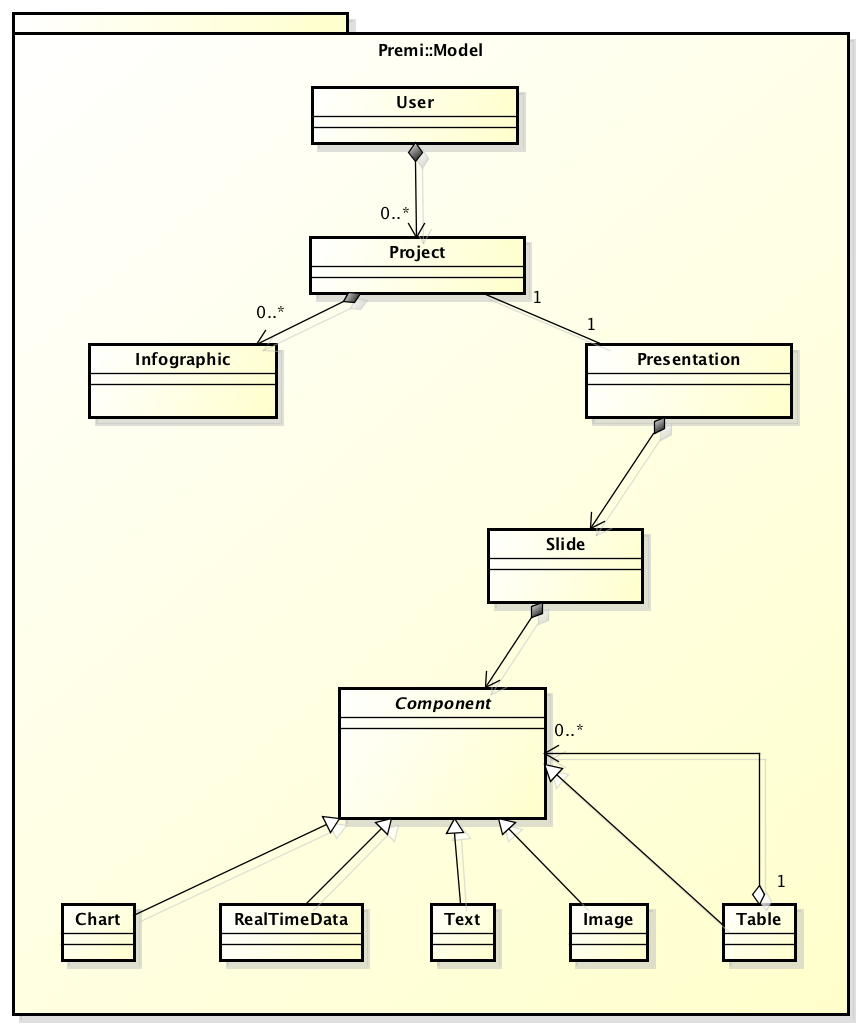
\includegraphics[width=0.7\linewidth]{img/premi_model}
		\caption[Premi::Model]{Premi::Model}
	\end{figure}
	
Il package gestisce lo scambio di informazioni tra una sorgente dati e l'interfaccia utente, attraverso i controller. Per ottenere informazioni si comunica con il model. Tutti i model comunicano tra di loro andando a costruire una serie di relazioni che rendono più semplice e veloce il recupero dei dati da parte del controller. Laravel utilizza un proprio ORM(Object Relational Mapping) chiamato Eloquent. Tutti i model estendono Eloquent che permette l'integrazione del database con il tipo di programmazione utilizzata.

	\newpage
\subsubsection{User}

	\begin{figure}[h]
		\centering
		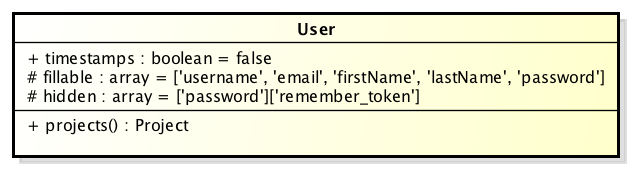
\includegraphics[width=0.7\linewidth]{img/User}
		\caption[Diagramma della classe User]{Diagramma della classe User}
		\label{fig:User}
	\end{figure}

	\subsubsection*{Descrizione}
	Il model User permette di gestire la collection users del database. Eloquent presume che il nome della classe sia il singolare del nome della collection nel database, quindi collega USer alla collection users.
	\subsubsection*{Utilizzo}
	Il model gestisce la collection users del database.
	\subsubsection*{Attributi}
	\begin{itemize}
		\item \textbf{+ timestamps : boolean = false :}\\
		Di default Eloquent automatizza l'inserimento del timestamp relativo all'inserimento e aggiornamento di un campo. Se alla variabile viene assegnato il valore le informazioni dell'inserimento e del aggiornamento non verranno aggiunto alla collection.
		\item \textbf{\# fillable : array = ['username', 'email', 'firstName', 'lastName', 'password']:}\\
		Quando si crea un model, si deve passare una serie di attributi al costruttore del model stesso. Questi attributi vengono assegnati al model tramite \textbf{mass assignment}. La propietà \textit{fillable} serve a specificare quali attributi devono essere assegnabili tramite il mass-assignment.
		\item \textbf{\# hidden : array = ['password', 'remember\_token''] : }\\
		La proprietà hidden si aggiunge quando si vuole limitare gli attributi che sono inclusi nel JSON.
	\end{itemize}
	\subsubsection*{Metodi}
	\begin{itemize}
		\item \textbf{+ projects() : Project}\\
		Abbiamo utilizzato la relazione embedsMany per riuscire ad incorporare il model projects all'interno dell'oggetto principale User. Il metodo ritorna Project su cui verrà chiamato il metodo save() nel caso in cui si voglia aggiornare il modello.
	\end{itemize}
	
\newpage
\subsubsection{Project}

%figura

	\subsubsection*{Descrizione}
	Il model Project rappresenta un progetto creato da un utente. Contiene la presentazio e una o
più infografiche create da esso o nessuna.

	\subsubsection*{Utilizzo}
	Viene utilizzato alla creazione o caricamento di un progetto.
	
	\subsubsection*{Attributi}
	\begin{itemize}
		\item \textbf{+ timestamps : boolean = false :}\\
		Di default Eloquent automatizza l'inserimento del timestamp relativo all'inserimento e aggiornamento di un campo. Se alla variabile viene assegnato il valore le informazioni dell'inserimento e del aggiornamento non verranno aggiunto alla collection.
		\item \textbf{\# fillable : array = [’name’]:}\\
		Quando si crea un model, si deve passare una serie di attributi al costruttore del model stesso. Questi attributi vengono assegnati al model tramite \textbf{mass assignment}. La propietà \textit{fillable} serve a specificare quali attributi devono essere assegnabili tramite il mass-assignment.
		\item \textbf{\# hiddem : array = ['password', 'remember\_token''] : }\\
		La proprietà hidden si aggiunge quando si vuole limitare gli attributi che sono inclusi nel JSON.
	\end{itemize}
	
	\subsubsection*{Metodi}
	\begin{itemize}
		\item \textbf{+ presentation() : Presentation}\\
		Abbiamo utilizzato la relazione embedsOne per riuscire ad incorporare il model Presentation all’interno dell’oggetto principale Project. Il metodo ritorna Presentation su cui verrà chiamato il metodo save() nel caso in cui si voglia aggiornare il modello.
		\item \textbf{+ infographics() : Infographics}\\
		Abbiamo utilizzato la relazione embedsMany per riuscire ad incorporare il model Infographic all’interno dell’oggetto principale Project. Il metodo ritorna Infographic su cui verrà chiamato il metodo save() nel caso in cui si voglia aggiornare il modello.
	\end{itemize}

\newpage
\subsubsection{Infographic}

%figure

	\subsubsection*{Descrizione}
	Questa classe rappresenta un’infografica di un progetto, ovvero una rappresentazione visuale della presentazione per mostrare in maniera semplice e veloce le informazioni.
	
	\subsubsection*{Utilizzo}
Viene utilizzata alla creazione di un’infografica di una presentazione.

\subsubsection*{Attributi}
	\begin{itemize}
		\item \textbf{+ timestamps : boolean = false :}\\
		Di default Eloquent automatizza l'inserimento del timestamp relativo all'inserimento e aggiornamento di un campo. Se alla variabile viene assegnato il valore le informazioni dell'inserimento e del aggiornamento non verranno aggiunto alla collection.
		\item \textbf{\# fillable : array = [’name’, ’path’]:}\\
		Quando si crea un model, si deve passare una serie di attributi al costruttore del model stesso. Questi attributi vengono assegnati al model tramite \textbf{mass assignment}. La propietà \textit{fillable} serve a specificare quali attributi devono essere assegnabili tramite il mass-assignment.
	\end{itemize}


\newpage
\subsubsection{Presentation}

	%figura

	\subsubsection*{Descrizione}
	Questa classe descrive la presentazione di un progetto. Contiene tutte le slide che servono a comporre la presentazione.

	\subsubsection*{Utilizzo}
	Viene utilizzato alla creazione o caricamento di una presentazione.
	
	\subsubsection*{Attributi}
	\begin{itemize}
		\item \textbf{+ timestamps : boolean = false :}\\
		Di default Eloquent automatizza l'inserimento del timestamp relativo all'inserimento e aggiornamento di un campo. Se alla variabile viene assegnato il valore le informazioni dell'inserimento e del aggiornamento non verranno aggiunto alla collection.
		\item \textbf{\# fillable : array = ['title']:}\\
		Quando si crea un model, si deve passare una serie di attributi al costruttore del model stesso. Questi attributi vengono assegnati al model tramite \textbf{mass assignment}. La propietà \textit{fillable} serve a specificare quali attributi devono essere assegnabili tramite il mass-assignment.
	\end{itemize}

	\subsubsection*{Metodi}
	\begin{itemize}
		\item \textbf{+ slides() : Slide}\\
		Abbiamo utilizzato la relazione embedsMany per riuscire ad incorporare il model Slide all’interno dell’oggetto principale Presentation. Il metodo ritorna Slide su cui verrà chiamato il metodo save() nel caso in cui si voglia aggiornare il modello.
	\end{itemize}
\newpage

\subsubsection{Slide}

	%figura

	\subsubsection*{Descrizione}
	Questa classe descrive una singola slide. Contiene tutti i gli oggetti appartenenti alla slide.
	
	\subsubsection*{Utilizzo}
Viene utilizzato alla creazione o caricamento di una slide.

	\subsubsection*{Attributi}
	\begin{itemize}
		\item \textbf{+ timestamps : boolean = false :}\\
		Di default Eloquent automatizza l'inserimento del timestamp relativo all'inserimento e aggiornamento di un campo. Se alla variabile viene assegnato il valore le informazioni dell'inserimento e del aggiornamento non verranno aggiunto alla collection.
		\item \textbf{\# fillable : array = [’xIndex’, ’yIndex']:}\\
		Quando si crea un model, si deve passare una serie di attributi al costruttore del model stesso. Questi attributi vengono assegnati al model tramite \textbf{mass assignment}. La propietà \textit{fillable} serve a specificare quali attributi devono essere assegnabili tramite il mass-assignment.
	\end{itemize}
	\subsubsection*{Metodi}
	\begin{itemize}
		\item \textbf{+ components() : Component}\\
		Abbiamo utilizzato la relazione embedsMany per riuscire ad incorporare il model Component all’interno dell’oggetto principale Slide. Il metodo ritorna Component su cui verrà chiamato il metodo save() nel caso in cui si voglia aggiornare il modello.
	\end{itemize}
\newpage

\subsubsection{Component}

	%figura

	\subsubsection*{Descrizione}
	Questa classe descrive la struttura genera di un componente.
	
	\subsubsection*{Utilizzo}
	Viene utilizzato alla creazione o caricamento di una componente.
	
	\subsubsection*{Attributi}
	\begin{itemize}
		\item \textbf{+ timestamps : boolean = false :}\\
		Di default Eloquent automatizza l'inserimento del timestamp relativo all'inserimento e aggiornamento di un campo. Se alla variabile viene assegnato il valore le informazioni dell'inserimento e del aggiornamento non verranno aggiunto alla collection.
		\item \textbf{\# fillable : array = [’type’, ’originX’, ’OriginY’, ’left’, ’top’, ’width’, ’height’, ’fill’, ’stroke’, ’strokeWidth’, ’strokeDashArray’, ’strokeLineCap’, ’strokeLine-Join’, ’strokeMiterLimit’, ’scaleX’, ’scaleY’, ’angle’, ’flipX’, ’flipY’, ’opacity’, ’shadow’, ’visible’, ’clipTo’, ’backgroundColor’, ’fillRule’, ’globalCompositeOperation']:}\\
		Quando si crea un model, si deve passare una serie di attributi al costruttore del model stesso. Questi attributi vengono assegnati al model tramite \textbf{mass assignment}. La propietà \textit{fillable} serve a specificare quali attributi devono essere assegnabili tramite il mass-assignment.
	\end{itemize}
	

\newpage
\subsubsection{Chart}

%figura

	\subsubsection*{Descrizione}
	Questa classe rappresenta la struttura di dati necessari per descrivere un grafico all’interno di una slide.
	
	\subsubsection*{Utilizzo}
Viene utilizzato alla creazione o caricamento di un grafico.

	\subsubsection*{Attributi}
	\begin{itemize}
		\item \textbf{+ timestamps : boolean = false :}\\
		Di default Eloquent automatizza l'inserimento del timestamp relativo all'inserimento e aggiornamento di un campo. Se alla variabile viene assegnato il valore le informazioni dell'inserimento e del aggiornamento non verranno aggiunto alla collection.
		\item \textbf{\# fillable : array = [’typeChart’ , ’data’]:}\\
		Quando si crea un model, si deve passare una serie di attributi al costruttore del model stesso. Questi attributi vengono assegnati al model tramite \textbf{mass assignment}. La propietà \textit{fillable} serve a specificare quali attributi devono essere assegnabili tramite il mass-assignment.
		
	\end{itemize}
	

\newpage
\subsubsection{RealTimeData}

%figura

	\subsubsection*{Descrizione}
	Questa classe rappresenta la struttura di dati necessari per descrivere RealTimeData (dato in tempo reale) all’interno di una slide.
	
	\subsubsection*{Utilizzo}
	Viene utilizzato alla creazione o caricamento di un RealTimeData.
	
	\subsubsection*{Attributi}
	\begin{itemize}
		\item \textbf{+ timestamps : boolean = false :}\\
		Di default Eloquent automatizza l'inserimento del timestamp relativo all'inserimento e aggiornamento di un campo. Se alla variabile viene assegnato il valore le informazioni dell'inserimento e del aggiornamento non verranno aggiunto alla collection.
		\item \textbf{\# fillable : array = ['pathParser’, ’pathFallback’, ’pathHandlerJs']:}\\
		Quando si crea un model, si deve passare una serie di attributi al costruttore del model stesso. Questi attributi vengono assegnati al model tramite \textbf{mass assignment}. La propietà \textit{fillable} serve a specificare quali attributi devono essere assegnabili tramite il mass-assignment.
		
	\end{itemize}
	
	
\newpage
\subsubsection{Text}

	%figura

	\subsubsection*{Descrizione}
	Questa classe rappresenta la struttura di dati di un campo di testo di una slide.
	
	\subsubsection*{Utilizzo}
	Viene utilizzato alla creazione o caricamento di un campo di testo.
	
	\subsubsection*{Attributi}
	\begin{itemize}
		\item \textbf{+ timestamps : boolean = false :}\\
		Di default Eloquent automatizza l'inserimento del timestamp relativo all'inserimento e aggiornamento di un campo. Se alla variabile viene assegnato il valore le informazioni dell'inserimento e del aggiornamento non verranno aggiunto alla collection.
		\item \textbf{\# fillable : array = [’text’, ’fontSize’, ’fontWeight’, ’fontFamily’, ’fontStyle’, ’lineHeight’, ’textDecoration’, ’textAlign’, ’textBackgroundColor']:}\\
		Quando si crea un model, si deve passare una serie di attributi al costruttore del model stesso. Questi attributi vengono assegnati al model tramite \textbf{mass assignment}. La propietà \textit{fillable} serve a specificare quali attributi devono essere assegnabili tramite il mass-assignment.

	\end{itemize}

\newpage
\subsubsection{Image}

	%figura

	\subsubsection*{Descrizione}
	La classe Image rappresenta la struttura dei dati necessari per rapresentare un’immagine all’interno di una slide.
	
	\subsubsection*{Utilizzo}
	Utilizzata quando viene inserita un’immagine per tenerne traccia.
	
	\subsubsection*{Attributi}
	\begin{itemize}
		\item \textbf{+ timestamps : boolean = false :}\\
		Di default Eloquent automatizza l'inserimento del timestamp relativo all'inserimento e aggiornamento di un campo. Se alla variabile viene assegnato il valore le informazioni dell'inserimento e del aggiornamento non verranno aggiunto alla collection.
		\item \textbf{\# fillable : array = [’src’, ’filters’, ’crossOrigin’, ’alignX’, ’alignY’,’meetOrSlice’, ’background’]:}\\
		Quando si crea un model, si deve passare una serie di attributi al costruttore del model stesso. Questi attributi vengono assegnati al model tramite \textbf{mass assignment}. La propietà \textit{fillable} serve a specificare quali attributi devono essere assegnabili tramite il mass-assignment.

	\end{itemize}

\newpage
\subsubsection{Table}

	%figura

	\subsubsection*{Descrizione}
	Questa classe rappresenta la struttura di dati di una tabella di una slide.
	
	\subsubsection*{Utilizzo}
	Viene utilizzato alla creazione o caricamento di una tabella.
	
	\subsubsection*{Attributi}
	\begin{itemize}
		\item \textbf{+ timestamps : boolean = false :}\\
		Di default Eloquent automatizza l'inserimento del timestamp relativo all'inserimento e aggiornamento di un campo. Se alla variabile viene assegnato il valore le informazioni dell'inserimento e del aggiornamento non verranno aggiunto alla collection.
		\item \textbf{\# fillable : array = [’row’, ’column’, ’title’, ’cellData’]:}\\
		Quando si crea un model, si deve passare una serie di attributi al costruttore del model stesso. Questi attributi vengono assegnati al model tramite \textbf{mass assignment}. La propietà \textit{fillable} serve a specificare quali attributi devono essere assegnabili tramite il mass-assignment.

	\end{itemize}